% Design Principles commented out — too generic, covered by intro and motivation

\section{\sys Design}

% Challenges C1/C2/C3 moved to §3 Motivation (sec:motivation-limitations)

\sys{} is designed to provide a safe, programmable, and workload-adaptive GPU resource management OS interface capable of supporting dynamic, AI-generated policies, transparent to applications. As identified in \S\ref{sec:motivation-limitations}, achieving these goals requires addressing three GPU-specific challenges unmet by existing CPU eBPF models: (1) cross-device latency that necessitates asynchronous policy execution, (2) tight coupling of memory and scheduling decisions demanding unified hooks across these domains, and (3) GPU device opacity requiring device-side verified BPF execution. The following subsections detail how \sys{} addresses these challenges.

\subsection{\sys{} Policy Execution Model}
\label{sec:design-interfaces}

\subsubsection{Programmable Lifecycle and Decoupled Execution}


\sys models GPU resource management as programmable lifecycles. GPU resources transition through defined lifecycles: memory chunks between activated, accessed, and evicted; compute contexts between created, scheduled, preempted and finished. 


To write a policy in \sys{}, Developers implement eBPF programs that attach to events in the lifecycle and direct state transitions using kernel functions (\emph{kfuncs}). In prior BPF extensibility systems, the primary effect is the \emph{return value}: the kernel asks a question at a transition point and the BPF program returns an answer (which CPU to dispatch to, whether to drop a packet). Triggers such as GPU faults, application-level API calls (uprobes), device-side execution events, and async tasks (bpf_wq) can each initiate multiple state transitions asynchronously, thereby decoupling policy triggers from their cross-device effects. This shift is forced by three properties of GPU policy: a single hook must produce multiple concurrent effects (e.g., prefetch and preempt simultaneously), effects must be asynchronous (DMA outlives the callback), and hooks span fundamentally different execution environments (host CPU, user process, GPU SIMT) where no unified return-value format is possible. 
This decoupling is not a design choice but a necessity forced by the cross-device boundary. Prior eBPF extensibility systems (sched\_ext, cache\_ext, XDP) each attach at a single subsystem, make synchronous decisions on local resources, and extend one domain at a time. In sched\_ext, the policy callback and the context switch it triggers execute on the same processor in the same microsecond; a 1:1 coupled model suffices. In \sys{}, the uprobe-triggered prefetch at \texttt{cudaLaunchKernel} initiates a DMA transfer that completes 6.6\,ms later on a different device, informed by device-side observations from a prior kernel execution, and may simultaneously preempt another tenant's context to free memory. No single synchronous callback at a single transition point can express this coordination across two devices, two domains, and two timescales.
These kfuncs express transitions along three structural dimensions: \emph{ordering} (evict chunk A before B), \emph{timing} (prefetch now rather than waiting), and \emph{selection} (preempt tenant X for Y). The kernel enforces safety by constraining policies strictly within these verified lifecycle operations.

\sys defines three eBPF program types to control distinct resource domains: \texttt{GPU_MEM} for memory placement, \texttt{GPU_SCHED} for scheduling decisions, and \texttt{GPU_DEV} for device-side execution. Memory placement is modeled as a programmable cache, exposing lifecycle events (\emph{activate}, \emph{access}, \emph{evict_prepare}, \emph{prefetch}) on GPU-managed units (e.g., 2MB UVM chunks). Policies implement transitions to reorder kernel-maintained eviction lists; safety invariants are kernel-enforced. Similarly, compute scheduling policies manage priority adjustments, and preemption. Device-side BPF handlers support fine-grained block scheduling (e.g., warp-level work-stealing decisions).


\begin{figure}[t]
\centering
\begin{tikzpicture}[
  node distance=0.4cm and 0.6cm,
  box/.style={draw, rounded corners, minimum height=0.6cm, minimum width=1.2cm, font=\small},
  trigger/.style={box, fill=blue!10},
  bpf/.style={box, fill=green!10},
  effect/.style={box, fill=orange!10},
  label/.style={font=\small\itshape, text=gray},
  arrow/.style={->, >=stealth, thick},
  dasharrow/.style={->, >=stealth, thick, dashed},
  every node/.style={font=\small},
]

% === sched_ext (top half) ===
\node[font=\small\bfseries] (sched_title) at (0, 0) {sched\_ext (coupled, 1:1, sync):};

\node[trigger] (s_trans) at (-2.5, -0.8) {transition};
\node[bpf]     (s_bpf)   at (0, -0.8)    {BPF};
\node[effect]  (s_eff)   at (2.8, -0.8)   {immediate effect};

\draw[arrow] (s_trans) -- (s_bpf);
\draw[arrow] (s_bpf)   -- (s_eff);

\node[label, below=0.05cm of s_trans] {point};
\node[label, below=0.05cm of s_eff] {same processor, same moment};

% === gpu_ext (bottom half) ===
\node[font=\small\bfseries] (gpu_title) at (0, -2.2) {\sys{} (decoupled, many:many, sync+async):};

% Triggers
\node[trigger] (t_a) at (-3.2, -3.2) {trigger A};
\node[trigger] (t_b) at (-3.2, -4.0) {trigger B};
\node[trigger] (t_c) at (-3.2, -4.8) {trigger C};
\node[trigger, fill=purple!10] (t_d) at (-3.2, -5.9) {trigger D};
\node[label, below=-0.05cm of t_d] {(device)};

% BPF + maps
\node[bpf, minimum height=1.8cm, minimum width=1.4cm] (g_bpf) at (-0.5, -4.0) {BPF\\+ maps};

% Effects (lifecycle transitions)
\node[effect] (e_x) at (2.8, -3.2) {transition X};
\node[label, right=0.05cm of e_x] {\scriptsize async, 6.6ms};
\node[effect] (e_y) at (2.8, -4.0) {transition Y};
\node[label, right=0.05cm of e_y] {\scriptsize ordering};
\node[effect] (e_z) at (2.8, -4.8) {transition Z};
\node[label, right=0.05cm of e_z] {\scriptsize from state};

% Arrows from triggers to BPF
\draw[arrow] (t_a) -- (g_bpf);
\draw[arrow] (t_b) -- (g_bpf);
\draw[arrow] (t_c) -- (g_bpf);
\draw[dasharrow] (t_d) -- (g_bpf);

% Arrows from BPF to effects
\draw[arrow] (g_bpf) -- (e_x);
\draw[arrow] (g_bpf) -- (e_y);
\draw[arrow] (g_bpf) -- (e_z);

% PCIe boundary
\draw[thick, dashed, gray] (-4.0, -5.4) -- (4.5, -5.4) node[right, font=\scriptsize\itshape, text=gray] {PCIe};

% Labels
\node[label] at (-3.2, -2.7) {triggers (open)};
\node[label] at (2.8, -2.7) {effects (lifecycle-bounded)};

% Lifecycle boundary box
\draw[thick, dotted, orange!60] (1.8, -2.9) rectangle (4.4, -5.1);
\node[font=\scriptsize, orange!80!black, rotate=90] at (4.6, -4.0) {lifecycle};

\end{tikzpicture}
\caption{Execution model contrast. In sched\_ext, each BPF callback makes one synchronous decision at one transition point (coupled, 1:1). In \sys{}, BPF programs triggered from any point in the GPU management stack can direct multiple lifecycle transitions asynchronously via kfunc effects (decoupled, many:many). Triggers are open; effects are lifecycle-bounded. The dashed line marks the host-device boundary.}
\label{fig:exec-model}
\end{figure}



More broadly, device-side BPF enables three distinct usage patterns beyond host-only extensibility: (1)~\emph{observation feedback}, where device handlers write warp-level statistics to cross-layer maps that host policies read (the expert frequency example above); (2)~\emph{combined host-device policy}, where device-side and host-side programs cooperate on the same transition (e.g., device L2 prefetch triggers host callback for extended prefetch); and (3)~\emph{device-local policy}, where device-side BPF makes scheduling decisions entirely on-device (e.g., work-stealing block scheduler via \texttt{should\_try\_steal}). The SIMT-aware verifier and cross-layer maps exist precisely to enable all three patterns.



\subsubsection{Example: MoE Expert Offloading}

We illustrate the model with MoE expert offloading, a scenario that naturally requires all three layers. Consider a 120B Mixture-of-Experts model (59\,GiB) on a 32\,GB GPU: not all expert weights fit in device memory, so the driver must continuously evict and migrate pages. Each token activates only a subset of experts, but the default driver uses LRU eviction and tree-based prefetching, which are unaware of expert activation patterns. The result: every token triggers page faults on cold expert pages, each incurring milliseconds of PCIe DMA stall.

A \sys policy addresses this with three cooperating BPF programs across three layers, connected by a shared map. First, during inference, a device-side BPF handler monitors which expert pages each warp actually accesses, writing per-expert access counts to a cross-layer map; this information is invisible to the host, as only device-side BPF can observe warp-level access patterns within GPU kernel execution. Second, a BPF program attached to \texttt{cudaLaunchKernel} fires before each layer executes; it reads the device-side access map to predict which experts the next layer will activate, then calls \texttt{bpf\_gpu\_prefetch\_async} to migrate their pages before compute begins, avoiding the 6.6\,ms fault-driven DMA stall by overlapping migration with computation. In multi-tenant settings, the same program can simultaneously preempt a low-priority tenant's GPU context via \texttt{gdrv\_sched\_preempt} to free device memory for the prefetch, illustrating how memory and scheduling are coupled: prefetch requires free memory, which requires a scheduling decision. Third, when memory pressure requires eviction, the driver invokes a BPF handler at the \emph{evict\_prepare} lifecycle event; the handler reads the same access-frequency map and applies LFU ordering, protecting frequently-activated expert pages and evicting cold ones first. The kernel enforces safety, including fallback FIFO eviction under pressure.

\begin{lstlisting}
// Device-side: observe expert access patterns
SEC("gpu_dev/mem_access")
int moe_observe(gdev_mem_access_ctx_t *ctx) {
  u64 va = ctx->va & EXPERT_MASK;
  u64 *freq = bpf_map_lookup_elem(&expert_freq, &va);
  if (freq) __sync_fetch_and_add(freq, 1);
  return 0;
}

// Uprobe: prefetch + preempt at kernel launch
SEC("uprobe/cudaLaunchKernel")
int moe_prefetch(struct pt_regs *ctx) {
  u64 next_va = predict_next_expert(ctx);
  // Memory: prefetch predicted hot experts
  bpf_gpu_prefetch_async(next_va, EXPERT_SIZE);
  // Scheduling: preempt BE tenant to free memory
  if (bpf_gpu_mem_pressure() > THRESHOLD)
    gdrv_sched_preempt(BE_CONTEXT);
  return 0;
}

// Driver hook: evict cold experts, protect hot ones
SEC("gpu_mem/evict_prepare")
int moe_evict(gdrv_mem_remove_ctx_t *ctx) {
  gmem_region_t *r = ctx->region;
  u64 *freq = bpf_map_lookup_elem(&expert_freq,
                                   &r->va);
  if (freq && *freq > HOT_THRESHOLD)
    bpf_gpu_move_tail(&ctx->evict_list, r); // keep
  else
    bpf_gpu_move_head(&ctx->evict_list, r); // evict
  return 0;
}
\end{lstlisting}

Each layer exists because information resides in a different place: expert activation patterns are visible only on the device, application-layer intent is visible only at API calls, and eviction and scheduling decisions are made inside the driver. The three BPF programs coordinate through cross-layer maps, directing lifecycle transitions across both memory and scheduling domains from triggers that span the entire stack.

\subsubsection{Policy Safety and Correctness Guarantees}



The policy capability surface equals the kfunc set: policies can only invoke approved lifecycle operations. This guarantees correctness (no invalid transitions, no memory corruption) but not performance isolation; a policy can flood async prefetches or starve eviction, degrading throughput, just as a sched\_ext policy can dispatch to the wrong CPU. The remedy is the same: unload and fallback. Regardless of where a BPF program is triggered, it can only direct valid lifecycle transitions through kfuncs; each kfunc validates its parameters and enforces lifecycle invariants before executing. The BPF verifier guarantees that programs terminate and stay within memory bounds. If a policy errs or is unloaded, the driver reverts to default behavior.

\subsection{High-Level Architecture}
\label{sec:arch}

\begin{figure}
\centering
    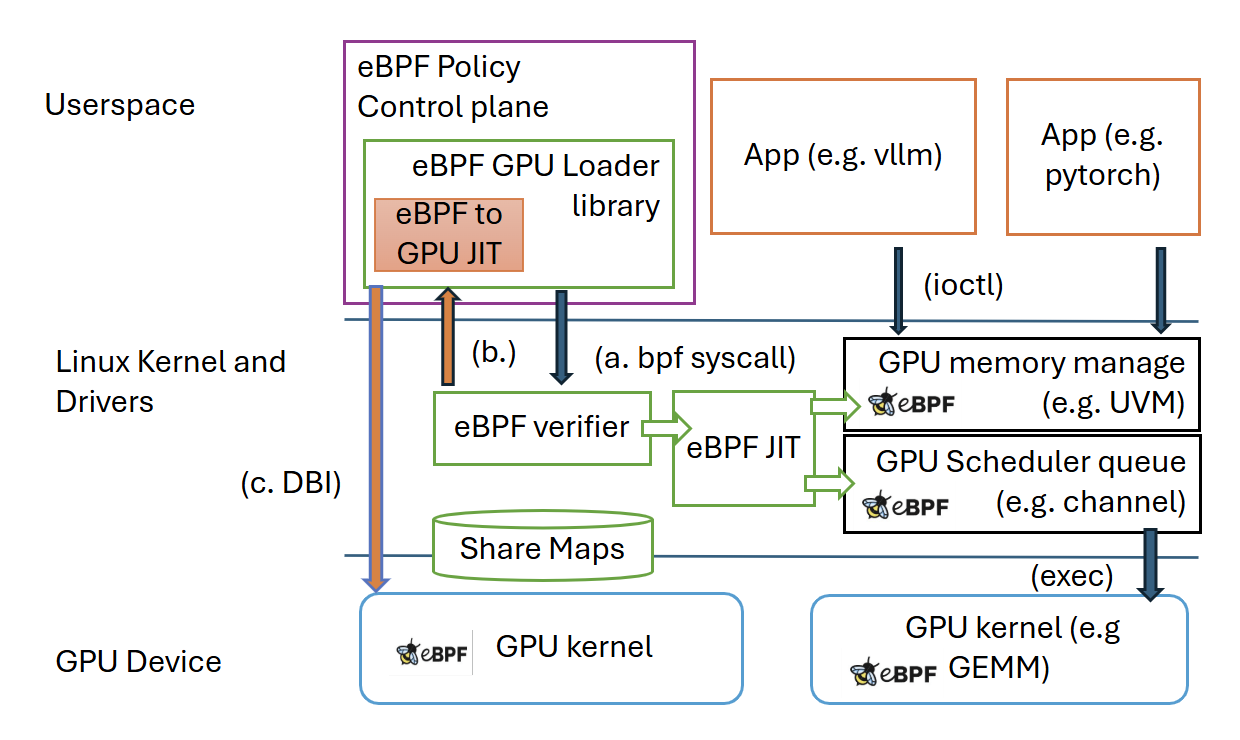
\includegraphics[width=\columnwidth]{img/gpu-ebpf-arch.png}
\vspace{-.5ex}
\caption{\sys architecture: cross-layer eBPF runtime spanning kernel driver and GPU device. The control plane deploys policies via (a) bpf syscall to verifier and driver hooks (b) GPU JIT after verification; (c) DBI injects trampolines into GPU kernels. Shared maps enable state coordination across layers.}
\label{fig:system-design}
\end{figure}

Figure~\ref{fig:system-design} shows how \sys realizes this execution model.

\paragraph{User-space Control Plane.}
Policy authors use standard eBPF tooling (e.g., \texttt{clang/libbpf}, \texttt{bpftool}) to build policy bytecode. The control-plane links against a loader library that installs policies and configures eBPF maps. It enables runtime policy redeployment and reconfiguration (e.g., eviction thresholds, sampling rates, priorities) without application or kernel restarts, and exports runtime metrics (e.g., region hotness, tenant latencies).

\paragraph{Host Driver and Device Runtime.}
\sys provides a unified runtime across host driver and GPU device contexts, managing verification, compilation, and map placement. It employs a SIMT-aware verifier (\S\ref{sec:verification}) that extends standard eBPF checks to verify warp-uniformity, SIMT control flow, and GPU synchronization constraints. Verified programs are JIT-compiled into native host code or GPU-compatible instructions (e.g., PTX). The runtime manages hierarchical logical eBPF map abstractions whose backing storage is automatically partitioned and replicated across host and device with consistency.
Policy execution occurs at structured hook points defined in GPU drivers and device. On the host, \sysdriver exposes \texttt{struct\_ops}-style hooks (e.g., region activate/eviction, GPU kernel scheduling). Host policies return concise policy decisions enforced via trusted kfuncs. On the GPU device, \sys injects trampolines at hook points and invokes device-side handlers at warp granularity. Device handlers update cross-layer maps with performance signals and make control decisions (e.g., prefetch, block-level scheduling) via trusted helpers that the runtime enforces.

\subsection{Runtime Verification and Optimizations}
\label{sec:verification}

\sys policies execute directly within privileged GPU driver and kernel contexts, making safety guarantees critical. We adopt a standard eBPF threat model: we trust system administrators loading policies, but consider policy code potentially buggy or misconfigured. The trusted computing base (TCB) includes the kernel and \sys kernel module, GPU compiler backend, and GPU driver/firmware. Policy authors only interact with eBPF and do not write native device code. For host-side verification, we reuse the existing Linux kernel eBPF verifier unchanged, relying on standard type-checking, bounded-loop, and memory-safety constraints. \sys-specific kfuncs and hooks are declared via BPF Type Format (BTF) metadata.

\subsubsection{SIMT-aware Verification}

Because the GPU executes in SIMT (Single Instruction, Multiple Threads) mode, device-side BPF programs must respect warp-level execution semantics. \sys introduces a SIMT-aware static verification model enforcing warp-level uniformity constraints to ensure efficient and safe GPU-side policy execution.
The key insight is that we distinguish \emph{warp-uniform} values (identical across warp threads, e.g., region identifiers) from \emph{lane-varying} values (thread-local GPU state). Policies may compute freely using lane-varying values, but these must not influence control-flow decisions or directly produce side effects visible outside a warp. To guarantee warp-level coherence, \sys mandates that branch conditions, loop bounds, and map-update keys be warp-uniform or derived via warp-level aggregation. Additionally, \sys prohibits GPU-wide barriers, global synchronization primitives, and non-uniform atomic operations, and imposes resource budgets per policy hook to bound memory and thread resource usage. These constraints ensure safe policy integration that respects GPU hardware execution semantics.

\subsubsection{Warp-level Execution Optimizations}

Direct scalar execution of eBPF after SIMT verification on GPU threads still causes resource overhead (e.g. duplicate memory update to maps) due to the SIMT. To resolve this, \sys introduces a warp-level aggregated execution model, executing policy logic once per warp using a designated "warp leader" (typically lane 0). Each hook invocation conceptually follows a two-phase approach: each lane independently computes lane-local contributions (e.g., effective addresses, counters) without influencing control flow or directly updating shared state. These contributions are then aggregated at warp granularity. Subsequently, the warp leader executes the policy handler once using aggregated inputs and warp-uniform context. The resulting decision is broadcast back to all lanes. This design minimizes GPU overhead while preserving eBPF's scalar semantics. To further reduce runtime overhead, \sys employs compiler-level optimizations (specialization and inlining) tailored for warp-level execution.

\subsubsection{Hierarchical Cross-layer Maps for State Coordination}

GPU policy decisions require coherent sharing of policy state across asynchronous CPU and GPU contexts. To transparently bridge CPU-GPU memory hierarchies, \sys introduces cross-layer maps. Logically, each map is a single unified key-value store accessible from host-side driver hooks, GPU-side device policies, and user-space control planes, and verifiable through eBPF's existing model. Physically, maps are realized as hierarchical shards across host DRAM, GPU global memory, and GPU-local storage (e.g., shared memory, SM-local). The runtime dynamically determines shard placement based on access frequency, latency, and capacity constraints. Following eBPF's soft-state philosophy, \sys maps provide relaxed, eventual consistency. Instead of strong global ordering, our runtime periodically merges GPU-local map shards into canonical snapshots at synchronization points, such as GPU kernel completion boundaries. This snapshot-based model is sufficient for policy decisions relying on approximate statistics. Occasional staleness affects decision optimality but cannot violate correctness invariants such as memory integrity, which remain enforced by the GPU driver and hardware MMU.
